\documentclass[12pt, a4, epsf] {article}
%==================================================
%Mypackages
\usepackage{epsf, amssymb, graphicx, epsfig, amsthm}
\usepackage[fleqn]{amsmath}
\usepackage{subfigure} % For subfigures
\usepackage{setspace} 
\usepackage{fancyhdr} 
\usepackage{eurosym}  %To write a Euro symbol
\usepackage[euler]{textgreek}
\usepackage[english]{babel}
\usepackage[utf8]{inputenc}
\usepackage[colorlinks = true, urlcolor = blue, linkcolor = blue]{hyperref}
\usepackage{graphicx}
\usepackage{float}
\usepackage{bbm}
\usepackage{placeins}
\usepackage{pdfpages}
\usepackage{listings}
\usepackage{tikz}
\usetikzlibrary{graphs,graphs.standard}
\usetikzlibrary{shapes.geometric}
\usetikzlibrary{trees}
\usepackage{forest}
\usepackage{pdfpages}
\usepackage{algorithm} 
\usepackage{algpseudocode} 
%\usepackage{refcheck}
%\usepackage[round]{natbib}


%Could change text height, width etc. 
\oddsidemargin 0mm
\evensidemargin 0mm
\textheight=24cm
\textwidth = 16cm
\topmargin= -1cm 

%Definition for theorems, definitions etc. for English texts
\theoremstyle{plain}
\newtheorem{theorem}{Theorem}[section]
\newtheorem{definition}[theorem]{Definition}
\theoremstyle{definition}
\newtheorem{example}[theorem]{Example}
\newtheorem{remark}[theorem]{Remark}


%==================================================
%My commands: Define your commands here:

\begin{document}
\begin{center}

{\Large \textbf{Epidemics on Transportation Networks}\\}
By Ho Lum Cheung, Dimas Muntesinos, Frank Acquaye, Elie Wanko \\
27 JUN 2020
\end{center}

\section*{Abstract}
\paragraph{}
Public transportation plays a vital role connecting people with each other. International trade and tourism is reliant on commercial aviation. And the most successful cities all have buses, trams, or subways connecting workers to their workplaces. However, the speed and connectivity of these transportation networks leave us vulnerable to the spread of diseases.\\
\paragraph{}
In this paper, we introduce a general agent-based framework for modeling disease propagation on transportation networks. We use it to build models of major transportation networks, and take a special look at the New York City subway to see how well the model can predict infection rate and infection hotspots during the 2020 COVID-19 epidemic.\\
\paragraph{}
Predicating contagion on subway lines, ridership at stations, commute time, and city-wide countermeasures, we were able to fit our model closely to empirical data. This suggests a correlation between these factors and the spread of COVID-19 and other ILI.

\section{Background}
\subsection{Epidemics and COVID-19}
\paragraph{}
Coronavirus disease 2019 (COVID-19) is a disease caused by the SARS-CoV-2 coronavirus. Since being identified in December 2019, it has been labelled by the WHO as a pandemic, and spread around the world. Epidemics such as the coronavirus have been a subject of research for centuries, and is of special interest to those working in public health. Recent waves of new research came in 2002 (SARS), 2009 (H1N1), and 2014 (Ebola). However, in these prior epidemics, researchers did not have access to as much data as we have currently. In recent years, the state of data science research tools has also greatly improved, allowing researchers to answer questions in novel ways, but following the scientific method.

\subsubsection{Mathematical Modeling of Epidemics}
\paragraph{}
There are two basic types of modeling for epidemics; statistical and mechanistic. While statistical modeling has typically given more accurate forecasts for a well-known situation, mechanistic models such as the SIR and SEIR compartmental models help to explain why phenomena such as epidemics spread the way they do, and what impact various policy decisions will have on the result.
\subsubsection{SEIR Model}
\paragraph{}
As we will be using the SEIR model\cite{hethcote_2000} in our research, we will cover it briefly here. The SEIR compartmental model is a mathematical modeling of infectious diseases where a closed population of people move successively from compartment to compartment (suspected to exposed to infected and to removed). We briefly provide an explanation of each compartment and leave the equations below.
\begin{itemize}
	\item \textbf{Susceptible (S)} - These people are susceptible to getting the disease from someone infected.
	\item \textbf{Exposed (E)} - These people are no longer susceptible to the disease, and do not infect others. After a latent period, they become infectious.
	\item \textbf{Infected (I)} - These people will spread the disease to susceptible people. After a period of time they are removed by recovery, hospitalization, death.
	\item \textbf{Removed (R)} - Sometimes known as resistant or recovered. We will do our modeling with the term 'removed'. These people are no longer spreading the disease.
	\item \textbf{Contact Rate ($\beta$)} - Rate at which infected people infect susceptible people.
	\item \textbf{Latent Rate ($\alpha$)} - Rate at which exposed people become infected.
	\item \textbf{Removal Rate ($\gamma$)} - Rate at which infected people become removed.
\end{itemize}
\begin{align*}
&S(t) + E(t) + I(t) + R(t) = N \\\\
&s(t) = S(t)/N, e(t) = E(t)/N, i(t) = I(t)/N, r(t) = R(t)/N \\\\
&ds/dt = - \beta * s(t) * i(t) \\\\
&de/dt = \beta * s(t) * i(t) - \alpha * e(t) \\\\
&di/dt = \alpha * e(t) - \gamma * i(t) \\\\
&dr/dt = \gamma * i(t) \\\\
\end{align*}
\paragraph{}
The system of equations described above can be numerically solved given $\beta,\alpha,\gamma$ and initial values $S(0),E(0),I(0),R(0)$. And if we have values for S,E,I,R at certain times, we can fit $\beta,\alpha,\gamma$ to better define the disease's epidemiological characteristics and predict its future course. Lastly, we note that $R_0$, an important characteristic known as the basic reproductive rate, can be calculated for the SEIR model as $\beta/\gamma$.
\subsubsection{Other Compartmental Models}
\paragraph{}
While we have done research into simpler and more advanced models and are interested in cases such as super-spreaders, we believe the SEIR model to be sufficient for our needs. Basic SIR is insufficient because public health officials often make policy decisions based on positive case numbers. For example, an official may decide to impose strict isolation only after 100 positive cases. But by the time there are 100 cases of 'infected' people, there may be 1000 exposed people who will meaningfully impact epidemic statistics.
\subsection{Epidemics on Transportation Networks}
\paragraph{}
Epidemics on transportation networks have been modeled in many different ways depending on the needs of the researcher. The most important differences are usually the type of transportation network, and the duration of interest, and a recurrent issue is modeling passenger flow. A popular motivation is exploring countermeasure policies. We highlight some prior research in the sections below.
\subsubsection{Flu on the London Underground \cite{gosce_johansson_2018}}
\paragraph{}
In this paper, the researchers modeled the "contact rate" of riders of the London Underground (subway system) by breaking down the stages of subway travel (entering, waiting, riding, exiting), and concluded that riders of some boroughs were at higher risk than riders from other boroughs. Their analysis was consistent with PHE data for influenza-like illnesses (ILI). The researchers also made additional observations such as that rush hour contributes to infection due to higher passenger density and longer waiting times.
\subsubsection{Time-dependent links in Singapore\cite{singapore_bus_2020}}
\paragraph{}
In this paper, which is a pre-publication as of June 1, 2020, the researchers modeled the Singapore bus system while limiting the spread of disease to passengers in the same location. They investigated various countermeasures such as reducing bus service and requiring personal protective equipment (PPE).
\subsubsection{Passenger Flow on the World Aviation Network\cite{mao_wu_huang_tatem_2015}}
\paragraph{}
In this paper, not directly related to epidemiology, the researchers proposed an open-source statistical modeling of passenger flow in the World Airline Network(WAN). This would be useful for modeling the spread of disease worldwide via aviation. It seems that while they were initially successful, their website and data are no longer available.
\subsubsection{Domestic Passenger Flow in Russia\cite{tutu_2020}}
\paragraph{}
In this blog post, Tutu, a Russian travel website, gathers, shares, and analyzes holistic passenger flow data (buses, trains, airplanes) across Russia. Treating Russia as a closed system due to closed borders, they estimate the start and end of the outbreak in Russian cities using an SIR epidemiological model.
\subsubsection{A Simulation of New York City\cite{cooley_brown}}
\paragraph{}
In this paper, the researchers make a very thorough model of New York City. While the title suggests they focused on subways, they modeled hospitals, schools, and major hubs with the subways delivering people to their places of work and education. They fit their work to historical flu data as well as infection numbers from prior work and also investigated the effect of countermeasures (interventions). They estimated that the subway was directly responsible for 12.5\% of all infections in NYC.
\subsubsection{Our Own Research}
\paragraph{}
In this paper, we focus on the NYC Subway. However, in the appendix we use our framework to model some other transportation networks to demonstrate the robustness of the framework, show similarities and differences between different types of transportation, and highlight key general facts about epidemics on transportation networks.
\subsection{Agent-Based Models}
\paragraph{}
An agent-based model(ABM) is a computational model used to simulate the overall effects of individual agents on a system. Some famous prior uses include Conway's Game of Life and Schelling's Segregation Model\cite{schelling_1971}. ABMs consist of one or several types of agents interacting with an environment. For example, in Schelling's Segregation Model, the agents have a race and a tolerance level (of other races). If the agent finds the surrounding environment intolerable, they will independently move away. Given certain hyper-parameters, segregated communities eventually form in this environment.
\paragraph{}
ABMs offer a number of benefits over traditional mathematical models. Complex systems which cannot be easily solved mathematically can be simulated. These simulations help policy makers make decisions when mathematical results are not available and real world experiments are impractical \cite{medicine_geller_ogawa_wallace_2015}. \\
\paragraph{}
For example, one popular use case of ABMs is in urban planning to simulate traffic flow. Given empirical traffic flow data, it is virtually impossible to calculate the optimal traffic light configuration for a city and extremely expensive to run multiple configuration experiments. However, ABM software with various vehicles as agents and the city traffic grid as the environment can easily find a satisfactory configuration \cite{traffic_book_2014}.
\subsection{COVID-19 in NYC}
\paragraph{}
In addition to general knowledge about COVID-19, it would behoove the reader to know about the early spread of the disease in New York. Analysis of viral RNA in patients at the Mount Sinai Health System has lead researchers to conclude that the virus first came into the community through "multiple, independent but isolated introductions" from Europe and elsewhere in the USA\cite{gonzalez_2020}. Below we have also given an approximate timeline of some of the most relevant events as of June 1st, 2020. We would also like to note that as forensic researchers begin examining the data, some significant new dates or corrections may arise:\\ 
\begin{itemize}
	\item February 25 - First positive test in NYC from a 39 year-old female healthcare worker flying back from Iran.
	\item March 3 - First confirmed P2P spread in NYC.
	\item March 9 - Mayor holds press conference and notes that there have been 16 confirmed cases.
	\item March 12 - Mayor declares a local state of emergency.
	\item March 15 - Schools officially close.
	\item March 22 - State order (PAUSE) to shelter in place comes into effect.
\end{itemize}
\subsection{COVID-19 and the NYC Subway}
On April 24th, 2020, a researcher at MIT released a working paper finding that "The Subways Seeded the Massive Coronavirus Epidemic in New York City"\cite{subway_epidemic_seed}. The paper received a lot of attention from the media. There is, at least, significant correlation between subway lines and severity of infection, but causation is heavily disputed. For example, high infection rate could be rated to dense housing, and housing is denser around subway stations. 

From this paper, and other prior research into subways, we bring into our own work two main ideas to test about disease spread on subways:\\
\begin{itemize}
	\item Infection on a subway network depends much more strongly on the line than the geographical distance or shortest path between stations.
	\item Infection on a subway network depends on the average commute time of commuters using the station.
\end{itemize}
\FloatBarrier
\subsection{Subway Nomenclature and Other Definitions}
\begin{itemize}
    \item {Station} - Passengers enter subway stations in order to ride the subway to an exit station.
    \item {Complex} - Multiple stations can reside in one station complex.
    \item {Turnstiles} - Barriers at the entrance and exit of stations which count people entering and exiting. 
    \item {Line} - The train tracks on which services and routes run.
    \item {Service/Route} - Trains follow specific routes between stations based on a timetable. 
    \item {Borough} - A geographical region. NYC has 5 boroughs. 
    \item {MODZCTA} - Modified Zip Code Tabulation Areas. They are very similar to zip (postal) codes, but are used due to postal codes sometimes not uniquely identifying geographical regions.
\end{itemize}
\section{Data Sources and Preprocessing}
\subsection{MTA Station Data \cite{mta_stations}}
\paragraph{}
This dataset has basic subway station information. It has stations, their longitude, latitude, associated complex (if any), line, route, and borough. We can find the MODZCTA from the longtitude and latitude data.\\
In this dataset, station 167 is listed twice, so we took care to combine the route data. We also split service 'S' into 3 different services as it represents 3 different shuttle services. We also split services on the 'A' line, into 3 different services depending on the destination. 
\subsection{MTA Turnstile Data \cite{mta_turnstiles}}
The MTA also publishes turnstile data with turnstiles reporting every 4 hours. However, we only need a basic picture of the daily in and out flow of each station, so we only process the aggregate passenger flow of each station between March 1 and March 21 (inclusive). 
\begin{figure}
    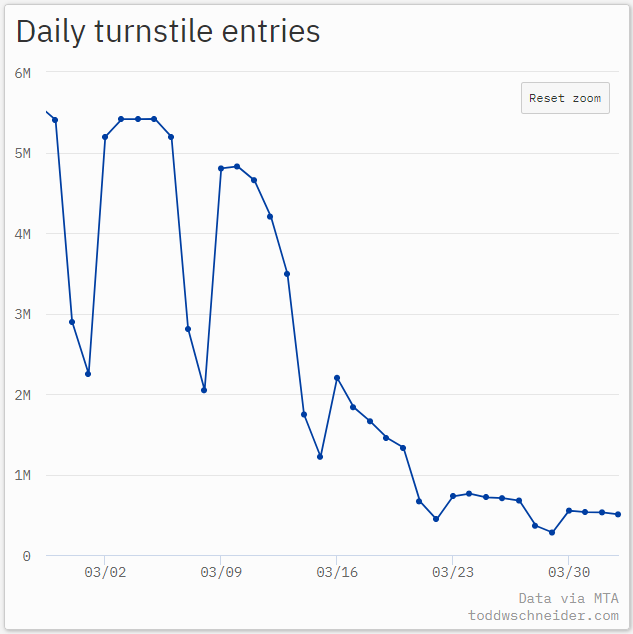
\includegraphics[width=6cm]{Scratch_Visuals/schneider_ridership.png}
    \caption{NYC Subway daily turnstile entries for March 2020 \cite{toddwschneider}}
\end{figure}
\subsection{NYC COVID-19 Data}
Since March 26, the NYC Health Department has been releasing and updating COVID-19 data on Github\cite{nychealth_2020}. Some data is incomplete or unavailable due to technical or privacy issues. For example, detailed case, death, and recovery numbers by MODZCTA only became available on May 18, 2020. However, a rudimentary record of positive tests for COVID-19 by modzcta has been available since April 1, 2020.
\section{Methodology}
\subsection{MESA\cite{Mesa}}
\paragraph{}
To implement our ideas, we chose to use MESA, an ABM framework written in Python. There are many other ABM frameworks, but many of them are oriented towards beginners and lacking features to organize the code necessary for complex behavior. Others are not suitable for modeling a complex environment (network). MESA provides a simple framework with basic Agent, Model, and Schedule classes from which we can specify the necessary behavior. In addition, our group already has a working knowledge of modeling networks using Python's NetworkX\cite{hagberg-2008-exploring}, which will be necessary for specifying the environment of our model.
\subsection{Modeling Framework}
\paragraph{}
Before focusing on the NYC subways, we built a general framework for modeling various transportation problems. This allowed us to see specifically how subways (and subway commuters) differ from other types of transportation networks. It also allows us to extend our initial research into other networks and environments. In the appendix, the reader will find some other models we have built and the key point behind the modeling. Below is a UML diagram of our framework.
\begin{figure}[htbp]
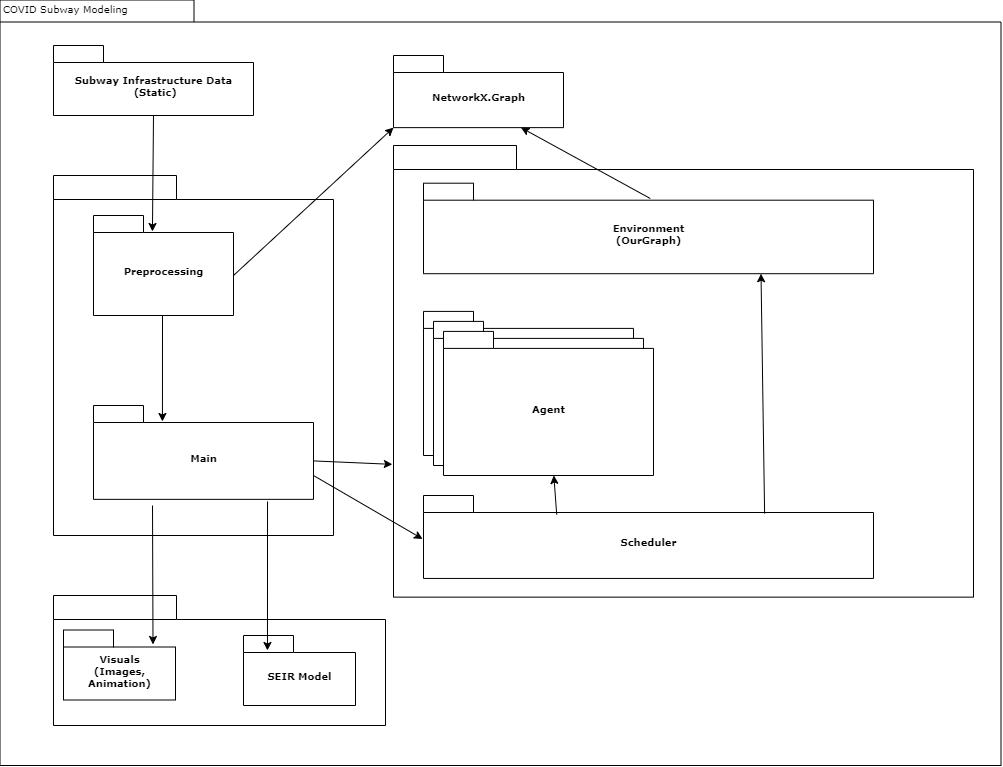
\includegraphics[width = 1.0\textwidth]{Scratch_Visuals/covid_subway.png}
\end{figure}
\subsection{SubwayModel}
This class inherits from the base TransportationModel. The main additional functionality is based on the model using SubwayAgents and a SubwayGraph to model the environment. It also has functionality related to deploying countermeasures given a certain threshold of infection. 
\subsubsection{SubwayAgent}
This class inherits from the base SEIRAgent and represents the population living around a specific subway station. The main additional property is the number of commuters, and the main additional functionality is adjustment of infection (and removal) rates based on exposure to the disease.
\subsubsection{SubwayGraph}
This class represents the environment of our agents. Each node represents a subway station. Each edge represents a connecting subway line or passage between stations. It is a wrapper around a NetworkX Graph with additional functionality.
\subsection{NetworkX\cite{hagberg-2008-exploring}}
This is a Python library used to model networks.
\subsection{Important Parameters, Hyper-parameters, and Values}
\subsubsection{Basic Epidemic Characteristics}
\begin{itemize}
    \item DEFAULT\_BETA - The default $\beta$ of the modeled disease in the SEIR model. It can be affected by countermeasures.
    \item DEFAULT\_GAMMA - The default $\gamma$ of the modeled disease in the SEIR model. It can be affected by countermeasures.
    \item DEFAULT\_ALPHA - The default $\alpha$ of the modeled disease in the SEIR model. It can be affected by countermeasures.
\end{itemize}
\subsubsection{Countermeasures}
\begin{itemize}
    \item ISOLATION\_COUNTERMEASURE - Models a government order to stay isolated after a certain number of people are infected. 
    \item RECOMMENDATION\_COUNTERMEASURE - Models a government recommendation to be safe after a certain number of people are infected. The isolation countermeasure supercedes this countermeasure.
    \item AWARENESS\_COUNTERMEASURE - Models increasing public awareness after a certain number of people are infected. As time passes since the public first becomes aware of a problem, the infection and removal rates decrease due to self-initiative.
\end{itemize}
\subsubsection{Values}
\begin{table}[htbp]
\begin{tabular}{|l|l|l|l|l|}
\hline
\textbf{Values} &
  \textbf{\begin{tabular}[c]{@{}l@{}}Contact\\ Rate ($\beta$)\end{tabular}} &
  \textbf{\begin{tabular}[c]{@{}l@{}}Latent\\ Rate ($\alpha$)\end{tabular}} &
  \textbf{\begin{tabular}[c]{@{}l@{}}Removal\\ Rate ($\gamma$)\end{tabular}} &
  \textbf{\begin{tabular}[c]{@{}l@{}}Start\\ Trigger\end{tabular}} \\ \hline
\textbf{Default Rates}                                                           & \textbf{1.75} & \textbf{0.2} & \textbf{0.5} & t = 0               \\ \hline
\textbf{\begin{tabular}[c]{@{}l@{}}Isolation\\ Modifier\end{tabular}}      & 0.25          & 1            & 2            & I \textgreater 5000 \\ \hline
\textbf{\begin{tabular}[c]{@{}l@{}}Recommendation\\ Modifier\end{tabular}} & 0.67          & 1            & 1.5          & I \textgreater 500  \\ \hline
\textbf{\begin{tabular}[c]{@{}l@{}}Awareness\\ Modifier\end{tabular}}      & 1 to 0.25     & 1            & 1            & I \textgreater 500  \\ \hline
\end{tabular}
\end{table}
These values were chosen to approximate the epidemiological characteristics of COVID-19. Other sources\cite{nyc_health_covid_summary}\cite{gonzalez_2020}\cite{ndairou_area_nieto_torres_2020}\cite{xu_mccluskey_cressman_2013} have investigated the best numbers more thoroughly, but for our modeling it is only necessary that the values are not preposterous (more than 200\% difference).\\
\subsubsection{Other Parameters}
We also used a number of other parameters.
\begin{itemize}
    \item Global Exposure Rate - This adds an additional infection chance based on globally infected. The value of 0.7 indicates that we think approximately 30\% of viral propagation is subway-based and the other 70\% is not subway based.
    \item Defiance - The local population will defy government orders if very few people are infected in their area.
    \item Awareness Increase Rate - Awareness increases by a negative exponential up to 0.75. The rate is calculated so that most of this gain is achieved in the first month.
    \item Borough Commuting Modifier - This modifier approximates the percent of the population which commutes by borough. This is in lieu of better research which estimates the percentage of commuters by station.
\end{itemize}
\subsection{Algorithm}
Below is a simplified algorithm for our model.
\begin{algorithm}
\caption{Simulation of Disease Spread on Subways}\label{euclid}
\begin{algorithmic}[1]
\For{$i=1; i < TIMESPAN; i++$}
    \State Check conditions (i, number of infected) to see if we should deploy COUNTERMEASURES
    \For{Station in SubwayModel.Environment.Nodes}
        \State Calculate 'Local Exposure' from locally infected and commute time.
        \State Calculate 'Route Exposure' from infected on the same route.
        \State Calculate 'General Exposure' due to city-wide infected.
        \State Update 'Exposure' At Station based on above conditions
    \EndFor
    \For{Agent in SubwayNetwork.Agents}
        \State Get 'Exposure' At Location
        \State Get City-wide COUNTERMEASURES
        \State Get Percentage of commuters
        \State Calculate SEIR beta and gamma based on conditions
        \State Update SEIR numbers
    \EndFor
\EndFor
\end{algorithmic}
\end{algorithm}
\FloatBarrier
\section{Fitting and Results}
\subsection{Fitting to SEIR}
We first fit overall SEIR numbers to NYC case, death, and recovery numbers. We only sought to fit the total cases to $I(t) + R(t)$ and adjusted the countermeasure properties to do so. Since we were at complete liberty to adjust these numbers, it is unsurprising that we created a near-perfect fit.\\
\begin{figure}[htbp]
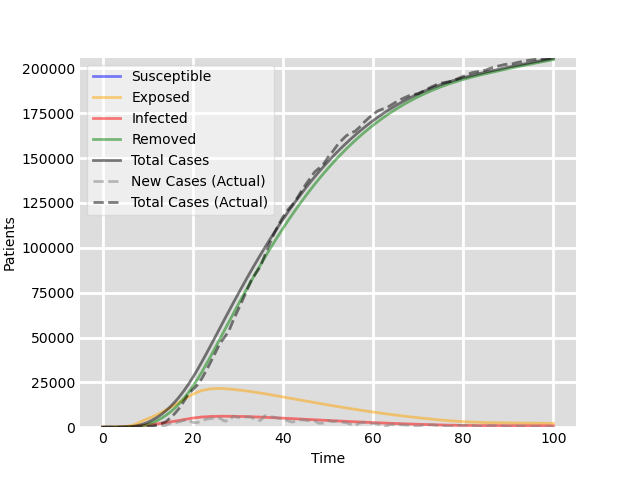
\includegraphics[width = 0.8\textwidth]{Scratch_Visuals/SEIR_Curve_NYC_3.png}
\caption{SEIR Fitting to NYC Case Total. \textit{MAPE ($t \geq 30$): 0.0145}}
\end{figure}
\FloatBarrier
\subsection{Fitting to MODZCTA}
Next we fit our data to MODZCTA. Due to the lack of numbers, we are only able to fit starting on April 1st (t=32). When calculating fitting error using MAPE, we exclude MODZTAs with no subway stations.
\begin{figure}[htbp]
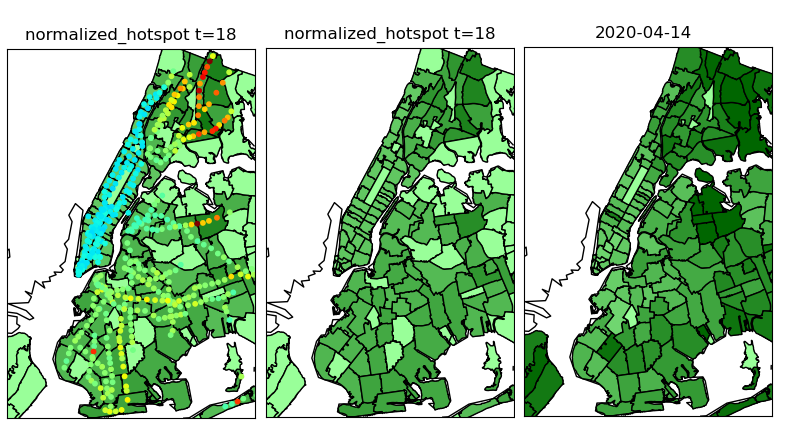
\includegraphics[width = 1.0\textwidth]{Scratch_Visuals/NYC_Geo_Fitting.png}
\end{figure}
\FloatBarrier
\begin{small}
Scale(0 - 0.11 infections/person, 0 - 0.11 infections/person, 0 - 0.20 cumulative cases/person) 
\end{small}
\FloatBarrier
\begin{small}
\textit{MAPE($t \geq 32, Stations \geq 1 = 0.311$)}\\
\end{small}
\FloatBarrier
A MAPE Of 0.311 is much worse than the overall error. But it still suggests that there is some correlation. We would expect that even with additional tuning and more granular subway data, there would be a large amount of error due to infection spread which cannot be modeled with currently available data.
\section{Further Research}
\subsection{Controlling for demographics}
\paragraph{}
While there is good correlation between empirical infection rates and our modeling, there is also likely to be good correlation between these rates and demographic data like population density and income. We have not tried to control for this.
\subsection{NYC: An open system}
\paragraph{}
Our research into New York City suggests that there is a significant amount of commuting from outside the 5 boroughs \cite{nyc_commuting}. In addition, we have not even considered Staten Island.
\subsection{Fitting to a different system}
\paragraph{}
We have not fit our research to a different subway system for a different city.
\subsection{Unnecessary hyper-parameters}
\paragraph{}
While we initially started with a minimal number of hyper-parameters, the model has become bloated with additional parameters which accommodate missing data and provide for a better fit. We should investigate ways to obtain or interpolate the data or question whether it is necessary to model it.
\section{Conclusion}
\paragraph{}
In this paper, we used a general agent-based framework to create a model for the spread of COVID-19 through New York City via the subway system. We took into account various important factors such as commute time, subway routes, and city-wide countermeasures in the model hyper-parameters and found a good fit for overall New York City case data.
\paragraph{}
Predicating contagion on these parameters, we were also able to closely match the empirical data by MODZCTA. This suggests a correlation between these factors and the spread of COVID-19 and other ILI.
\nocite{*}
\bibliography{bib_file}{}
\bibliographystyle{unsrt}
\section{Appendix}
\subsection{Additional Models}
\subsubsection{Madrid Commuter Rail}
\paragraph{Data}
\begin{itemize}
    \item Madrid Cercanias Routing Data \cite{Madrid_Cercanias_Routing_Data}
    \item Madrid Cercanias Turnstile Data \cite{Madrid_Cercanias_Turnstile_Data}
\end{itemize}
\paragraph{Methodology}
\begin{enumerate}
    \item Determine in and out flow weights for each station
    \item Model trains running on the network
    \item Model passengers entering, waiting, riding, exiting
    \item Model passengers infecting passengers at the same location
    \item Analyze infection rates and locations
\end{enumerate}
\paragraph{Result}
\begin{figure}[htbp]
Our results show that the central hub at Madrid is the most dangerous station, and that most infections happen during Madrid's rush hours.
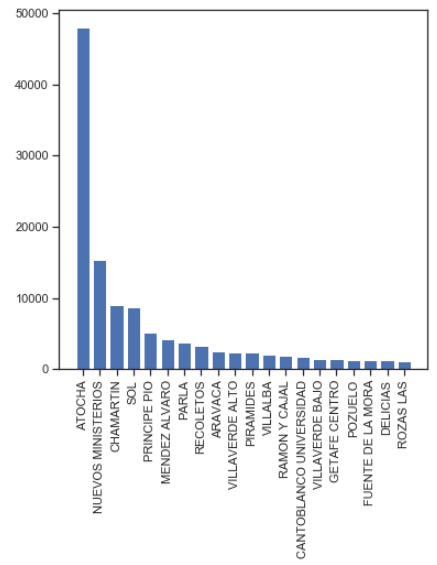
\includegraphics[width=0.8\linewidth]{Scratch_Visuals/madrid-cercanias-stats-top20.png}
\end{figure}
\begin{figure}[htbp]
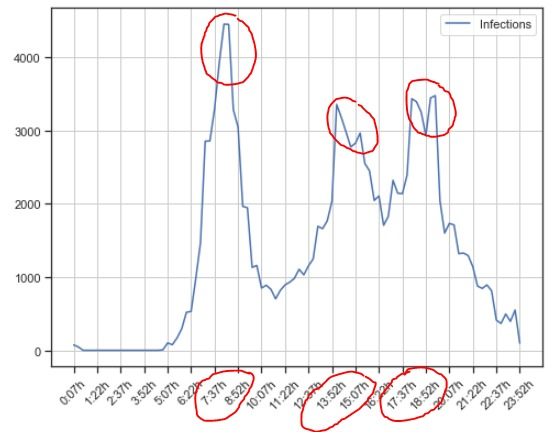
\includegraphics[width=0.8\linewidth]{Scratch_Visuals/madrid-infection-timeline.jpg}
\end{figure}

\subsubsection{World Airline Network}
\paragraph{Data}
\begin{itemize}
    \item List of Airports - OpenFlights \cite{openflights}
    \item List of Air Routes - OpenFlights \cite{openflights}
    \item Airport Passenger Flow Numbers - \cite{airport_traffic}
    \item Top Air Routes \cite{airport_pairs}
    \item Other Air Routes
\end{itemize}
\paragraph{Methodology}
\begin{enumerate}
    \item Process airports, air routes
    \item Add all known passenger flow numbers
	\item Add all known airport and air route labels
	\item Classify remaining airports and air routes
	\item Interpolate missing air route data 
\end{enumerate}
\paragraph{Result}
Our results show that with accurate passenger flow data and labeling, it's possible to show the idea that diseases have a domestic and international wave.
\FloatBarrier
\begin{figure}[htbp]
    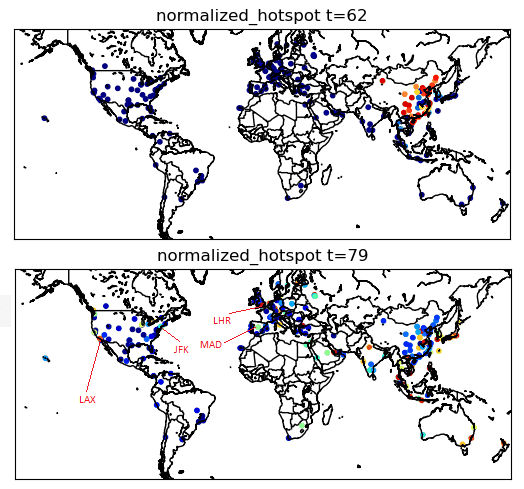
\includegraphics[width=1.0\textwidth]{Scratch_Visuals/covid_airlines.png}
\end{figure}
\end{document}
